%%% PLOT FILE - Group measures condition
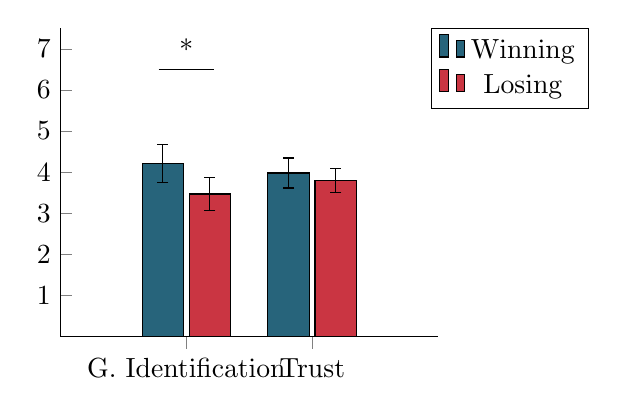
\begin{tikzpicture}%
\begin{axis}[%
    ybar,
    %title=Test,%
    axis y line*=left, axis x line*=bottom,%
    ymin=0,
    ymax=7.5,
    ytick={1,2,...,7},
    legend style={at={(1.4,1)}},
    %x tick label style={rotate=45,anchor=east},%
    symbolic x coords={G. Identification,Trust},%
    xtick=data,
    enlarge x limits=1,
    bar width=15pt,
    height=5.5cm,
    %ylabel=difference in \%,%
        ]%
\addplot+[%
    color=black, %
    fill={rgb,255:red,39; green,100; blue,123},%
    %postaction={pattern= north east lines},
    error bars/.cd,%
    y dir=both,%
    y explicit,%
        ]%
coordinates {
            (G. Identification,4.22) +- (G. Identification,0.464)
            (Trust,3.98) +- (Trust,0.365)
        };%
\addplot+[
    color=black,
    fill={rgb,255:red,202; green,53; blue,66},%
    error bars, y dir=both, y explicit]
				coordinates {
				(G. Identification,3.47) +- (G. Identification,0.407)
				(Trust,3.79) +- (Trust,0.291)};
    
\draw (axis cs:G. Identification,6.5) ++ (-10pt,0pt) -- ++(20pt,0pt);
\node[anchor=south] at (axis cs:G. Identification,6.5) {*};

\legend{Winning,Losing}
\end{axis}%
\end{tikzpicture}%